\documentclass{article}
\usepackage{graphicx}
\usepackage{amsmath}
\usepackage[style=ieee]{biblatex} % Establecer el estilo de las referencias como IEEE
\usepackage{xcolor}
\usepackage{hyperref}
\usepackage{titletoc}
\usepackage{adjustbox}

\hypersetup{
    colorlinks=true,
    linkcolor=blue, % Color del texto del enlace
    urlcolor=blue % Color del enlace
}

\usepackage{longtable} % Agrega el paquete longtable

\definecolor{mygreen}{RGB}{0,128,0}

\usepackage{array} % Para personalizar la tabla
\usepackage{booktabs} % Para líneas horizontales de mejor calidad
\usepackage{graphicx} % Paquete para incluir imágenes
\usepackage{float}

% Definir márgenes
\usepackage[margin=1in]{geometry}

\renewcommand{\contentsname}{\textcolor{mygreen}{Tabla de Contenidos}}
\renewcommand{\figurename}{Figura}

\begin{document}

\begin{titlepage}
    \centering
    % Logo de la Universidad
    
\includegraphics[width=0.48\textwidth]{logo_universidad.png}
    \par\vspace{2cm}

    % Nombre de la Universidad y detalles del curso
    {\Large \textbf{Universidad Nacional de Colombia} \par}
    \vspace{0.5cm}
    {\large Ingeniería de Sistemas y Computación \par}
    {\large 2025966 Lenguajes de Programación (02)\par}
    \vspace{3cm}
    % Detalles del laboratorio y actividad
    {\large \textbf{Tarea 11} \par}
    {\large Computación cuántica: Implementación del algoritmo de búsqueda de Grover \par}
    \vspace{3cm}
    % Lista de integrantes
    {\large \textbf{Integrantes:} \par}
    \vspace{0.5cm}
    \begin{tabular}{ll}
    Javier Andrés Tarazona Jiménez & jtarazonaj@unal.edu.co \\
    Juan Sebastian Muñoz Lemus & jumunozle@unal.edu.co \\
    \end{tabular}
    \par\vspace{3cm}

    % Fecha
    {\large Mayo 12 de 2025 \par}
\end{titlepage}

\tableofcontents % Inserta la tabla de contenidos

\newpage % Salto de página para separar la tabla de contenidos del contenido del documento

% Contenido del artículo----------------------------------------------------------

%---------------------------------------------------------------------------------
% Intro --------------------------------------------------------------------------
%---------------------------------------------------------------------------------

\section{Introducción}\label{sec:intr}

En la computación clásica, la búsqueda en una base de datos no estructurada de $N$ elementos requiere en promedio $O(N)$ operaciones. Este proceso puede resultar ineficiente cuando se trata de grandes volúmenes de datos. En cambio, la computación cuántica ofrece nuevas perspectivas para resolver este tipo de problemas gracias a su capacidad de paralelismo cuántico y manipulación de estados en superposición.

El algoritmo de búsqueda de Grover, desarrollado por Lov Grover en 1996, permite encontrar un elemento marcado (o solución) dentro de un conjunto no estructurado con una complejidad de $O(\sqrt{N})$, lo que representa una mejora cuadrática significativa respecto a cualquier algoritmo clásico conocido.

Este proyecto busca implementar dicho algoritmo utilizando el \textbf{SDK Qiskit} y ejecutar el programa en uno de los computadores cuánticos disponibles a través de IBM Quantum Experience, con el fin de verificar su funcionamiento y estudiar su comportamiento frente a diferentes tamaños de entrada.

%---------------------------------------------------------------------------------
% Marco Teórico ------------------------------------------------------------------
%---------------------------------------------------------------------------------

\section{Marco Teórico}\label{sec:marc}

\subsection*{¿Cómo funcionan los computadores cuánticos?}

Un computador tradicional ejecuta algoritmos secuenciales utilizando una unidad de procesamiento clásico (CPU). En cambio, un computador cuántico emplea una unidad de procesamiento cuántico (QPU) para ejecutar circuitos cuánticos.

Para programar estos dispositivos, se pueden usar lenguajes como Python junto con frameworks que permiten interactuar con el hardware cuántico. Entre los más utilizados están Qiskit (desarrollado por IBM) y Cirq (de Google). En este curso se utilizará Qiskit como herramienta principal para diseñar y ejecutar algoritmos cuánticos.

\subsection*{¿Qué es un Qubit?}

Un qubit (bit cuántico) es la unidad básica de información en computación cuántica. A diferencia del bit clásico que puede tomar únicamente los valores 0 o 1, un qubit puede tomar simultáneamente ambos valores gracias al principio de superposición.

Cuando se mide un qubit, su estado colapsa y toma uno de los dos valores clásicos (0 o 1). El estado de un qubit se puede visualizar mediante la esfera de Bloch, donde:

\begin{itemize}
    \item Si el vector apunta hacia arriba, el qubit está en el estado $\vert 0 \rangle$.
    \item Si apunta hacia abajo, está en el estado $\vert 1 \rangle$.
    \item Cualquier otra dirección representa un estado en superposición.
\end{itemize}

La probabilidad de que colapse a 0 o 1 depende de la orientación del vector:

\begin{itemize}
    \item Si el vector apunta cerca del polo norte ($\vert 0 \rangle$), es más probable que colapse a 0.
    \item Si apunta hacia el ecuador de la esfera, hay un 50\% de probabilidad de obtener 0 y 50\% de obtener 1.
\end{itemize}

Desde un punto de vista matemático, el estado de un qubit se representa como un vector con dos componentes complejas:

\[
|\psi\rangle = \alpha \vert 0 \rangle + \beta \vert 1 \rangle \quad \text{representado como } [\alpha, \beta]
\]

donde:
\begin{itemize}
    \item $\alpha$: amplitud para colapsar a 0,
    \item $\beta$: amplitud para colapsar a 1,
    \item Las probabilidades de medición se obtienen como $|\alpha|^2$ y $|\beta|^2$,
    \item Propiedad fundamental: $|\alpha|^2 + |\beta|^2 = 1$.
\end{itemize}

\subsection*{Sistemas de más de un Qubit}

Cuando se tienen 2 qubits, existen 4 combinaciones clásicas posibles: 00, 01, 10 y 11. En un sistema cuántico, también existe el fenómeno del entrelazamiento cuántico, que permite estados complejos que no pueden separarse en qubits individuales.

Así, el estado cuántico de 2 qubits se representa con un vector de 4 amplitudes, una para cada combinación clásica. Para un sistema de $n$ qubits, se requiere un vector de $2^n$ componentes para describir el estado completo del sistema.

Este crecimiento exponencial permite que los computadores cuánticos sean especialmente potentes para ciertas tareas. Sin embargo, también impone retos técnicos y teóricos importantes relacionados con la manipulación y el control de sistemas cuánticos de múltiples qubits.

\subsection*{Puertas Cuánticas}

\subsubsection*{Puerta X (NOT cuántica)}

Esta es la versión cuántica de la puerta NOT clásica. Su función es intercambiar los valores del qubit:

\begin{itemize}
    \item Si el qubit está en el estado $\vert 0 \rangle$, pasa a $\vert 1 \rangle$.
    \item Si está en $\vert 1 \rangle$, pasa a $\vert 0 \rangle$.
\end{itemize}

Su representación matricial es:

\[
X = \begin{bmatrix} 0 & 1 \\ 1 & 0 \end{bmatrix}
\]

Para aplicar la puerta, se multiplica la matriz $X$ por el vector de estado del qubit.

Nota: Si se tienen múltiples qubits, la puerta $X$ se aplica solo al qubit seleccionado, y la matriz total se expande usando el producto tensorial.

\subsubsection*{Puerta Hadamard (H)}

Esta puerta transforma un estado definido (como $\vert 0 \rangle$ o $\vert 1 \rangle$) en una superposición cuántica. Su matriz es:

\[
H = \frac{1}{\sqrt{2}} \begin{bmatrix} 1 & 1 \\ 1 & -1 \end{bmatrix}
\]

Aplicando $H$ al estado $\vert 0 \rangle$ se obtiene:

\[
\vert \psi \rangle = \frac{1}{\sqrt{2}}(\vert 0 \rangle + \vert 1 \rangle)
\]

Esto significa que el qubit tiene 50\% de probabilidad de colapsar a 0 y 50\% de colapsar a 1 al ser medido.

En general, las operaciones cuánticas se implementan mediante multiplicación de matrices. Aunque estas operaciones son costosas para un computador clásico, los ordenadores cuánticos las realizan físicamente y en paralelo, aprovechando las propiedades de los qubits reales.

\subsection*{La compuerta Cuántica Z}

La compuerta Z es una compuerta cuántica unitaria que no altera la probabilidad de 
colapso del qubit, pero sí cambia su fase cuántica cuando se encuentra 
en el estado \(|1\rangle\). Matemáticamente, se representa como:

\[
Z = \begin{bmatrix} 1 & 0 \\ 0 & -1 \end{bmatrix}
\]

\begin{itemize}
    \item Si el qubit está en \(|0\rangle\), no hay efecto.
    \item Si está en \(|1\rangle\), el signo de la amplitud cambia a negativo.
    \item Esta operación es clave en algoritmos como Grover, ya 
            que permite invertir la fase de estados específicos como parte del proceso 
            de amplificación.
\end{itemize}

\subsection*{Z multi-controlada (MCMT)}

Una Z multi-controlada aplica la compuerta Z únicamente si una combinación específica 
de qubits de control está en el estado deseado (por lo general, todos en \(|1\rangle\)).

Esto permite cambiar el signo de la amplitud de un solo estado objetivo dentro de una 
superposición cuántica, sin afectar a los demás.

\begin{itemize}
    \item En Qiskit, se puede construir con la función \texttt{MCMT(ZGate(), num\_ctrls, 1)}.
    \item Se rodea de compuertas X cuando se quiere controlar sobre ceros.
    \item Esta técnica es fundamental para construir oráculos cuánticos que ``marcan'' 
            las soluciones dentro del espacio de búsqueda en algoritmos como Grover.
\end{itemize}

\subsection*{Teleportación Cuántica}

La teleportación cuántica es un protocolo que permite transferir el estado cuántico de un qubit a otro qubit distante, sin mover físicamente el qubit original.

\subsubsection*{¿Cómo funciona?}

\begin{enumerate}
    \item Dos personas (Alice y Bob) comparten un par de qubits entrelazados.
    \item Alice tiene un qubit adicional en un estado desconocido $\vert \psi \rangle$ que desea enviar a Bob.
    \item Alice realiza una medición conjunta entre su qubit desconocido y su parte del par entrelazado.
    \item El resultado de esa medición se envía a Bob por un canal clásico (por ejemplo, un mensaje de texto).
    \item Bob, con esa información, aplica una puerta cuántica a su qubit para transformarlo en el estado original $\vert \psi \rangle$.
\end{enumerate}

Es importante aclarar que no se transmite información más rápido que la luz ya que se requiere 
comunicación clásica. También el estado original se destruye en Alice al ser medido, respetando 
el principio de no-clonación cuántica. El protocolo 
no transporta materia ni energía, solo el estado cuántico.

\subsection*{Oráculo Cuántico}

Un oráculo cuántico en el algoritmo de Grover es una operación diseñada 
para marcar uno o varios estados cuánticos como soluciones. Técnicamente, se aplica una 
compuerta Z (cambio de fase) únicamente cuando el sistema se encuentra en el estado deseado.

Esto no altera las probabilidades directamente, pero 
multiplica la amplitud del estado marcado por $-1$, lo cual permite que, tras aplicar 
el difusor, la amplitud (y por ende la probabilidad) de esos estados se amplifique.

El oráculo actúa como una función booleana oculta $f(x)$, que devuelve 1 solo para 
los estados solución, y es implementada como un circuito cuántico reversible.

\subsection*{Transpilación}

Antes de ejecutar un circuito cuántico en un backend (procesador físico o simulador), 
se requiere adaptar el circuito a la arquitectura específica del dispositivo. 
A este proceso se le llama transpilación.

Incluye:
\begin{itemize}
    \item Reemplazar compuertas lógicas abstractas por compuertas físicas compatibles.
    \item Optimizar el orden y tipo de operaciones.
    \item Ajustarse a la conectividad de los qubits físicos.
\end{itemize}

Es el equivalente a pasar de una arquitectura lógica a una arquitectura física 
(clásica a cuántica).

\subsection*{Qiskit Primitives}

Los primitives en Qiskit son una interfaz de alto nivel para ejecutar tareas 
cuánticas comunes de forma modular y eficiente. Se utilizan especialmente en algoritmos 
modernos como Grover, VQE o QAOA.

Primitivas principales:
\begin{itemize}
    \item Sampler: ejecuta un circuito y devuelve una 
            distribución de probabilidad de los estados medidos.
    \item Estimator: calcula el valor esperado de un observable cuántico 
            sobre el estado generado por un circuito.
\end{itemize}

Estas primitivas son ideales para sistemas en la nube o simuladores locales, 
ya que abstraen los detalles técnicos y permiten enfocarse en la lógica del algoritmo.


\subsection{Contextualización del problema}

La computación cuántica ofrece ventajas significativas frente a la computación clásica en ciertos tipos de problemas, especialmente en tareas de búsqueda no estructurada. En este contexto, el \textbf{algoritmo de Grover} destaca por reducir el tiempo de búsqueda de $O(N)$ a $O(\sqrt{N})$, demostrando una mejora cuadrática.

Gracias a herramientas como \textbf{Qiskit} y el acceso a hardware cuántico real mediante plataformas como IBM Quantum, es posible implementar y probar este tipo de algoritmos. Este trabajo se enfoca en la implementación del algoritmo de Grover como un caso de estudio práctico que permite explorar las capacidades actuales de la computación cuántica y su potencial para resolver problemas complejos de manera más eficiente.


%---------------------------------------------------------------------------------
% Descripción y Justificación del Problema a Resolver ----------------------------
%---------------------------------------------------------------------------------

\section{Descripción y Justificación del Problema a Resolver}\label{sec:descr}

Buscar eficientemente un elemento dentro de una gran base de datos no estructurada es un problema central en muchas aplicaciones prácticas: desde motores de búsqueda, hasta problemas de satisfacibilidad y optimización. Si bien los ordenadores clásicos han sido capaces de abordar estos problemas, el tiempo requerido puede crecer exponencialmente con el tamaño de los datos.

El algoritmo de Grover demuestra una de las ventajas fundamentales de la computación cuántica: la posibilidad de realizar búsquedas de manera significativamente más rápida, sin requerir estructuras de datos específicas ni ordenamientos previos. Esta propiedad lo convierte en un caso de estudio ideal para experimentar con computadores cuánticos actuales, limitados en capacidad, pero suficientemente potentes para ejecutar este tipo de algoritmos.

La elección de Qiskit como entorno de desarrollo y de IBM Quantum como plataforma de ejecución responde a su accesibilidad, documentación robusta y a que permite la ejecución en hardware cuántico real.

\subsection{Objetivo Principal}

Implementar y ejecutar el algoritmo de búsqueda de Grover utilizando Qiskit sobre un computador cuántico de IBM, con el fin de analizar su rendimiento, validarlo empíricamente y comparar su comportamiento teórico y práctico.

\section{Diseño de la solución}\label{sec:dis}

El diseño del algoritmo de Grover parte de la necesidad de amplificar la probabilidad del estado objetivo dentro de una superposición cuántica de múltiples estados. Para lograr esto, se estructura el circuito cuántico en tres bloques fundamentales:

\begin{enumerate}
    \item \textbf{Inicialización:} Se parte de un registro de $n$ qubits, cada uno preparado inicialmente en el estado base $\vert 0 \rangle$. Luego, se aplica una compuerta Hadamard ($H$) a cada qubit para generar una superposición uniforme de los $2^n$ posibles estados.

    \item \textbf{Oráculo cuántico:} Es un circuito que identifica el estado objetivo $\vert x \rangle$ mediante un cambio de fase. Este oráculo actúa como una función $f(x)$ tal que:
    \[
    f(x) = \begin{cases}
    1 & \text{si } x = x_{objetivo} \\
    0 & \text{en otro caso}
    \end{cases}
    \]
    y realiza la transformación:
    \[
    \vert x \rangle \rightarrow (-1)^{f(x)} \vert x \rangle
    \]

    \item \textbf{Difusor o operador de inversión sobre la media:} Este bloque amplifica la amplitud del estado marcado mediante una inversión de las amplitudes alrededor del promedio de todas las amplitudes. Se construye aplicando Hadamard a todos los qubits, seguido de una compuerta de fase en el estado $\vert 0 \rangle$, y luego otra vez Hadamards.

    \item \textbf{Iteración de Grover:} La aplicación secuencial del oráculo y el difusor constituye una iteración del algoritmo. 
    El número óptimo de iteraciones se calcula en función del número total de estados posibles ($N = 2^n$) y del número de soluciones marcadas ($M$), mediante la siguiente expresión:

    \[
    r \approx \left\lfloor \frac{\pi}{4 \cdot \arcsin\left( \sqrt{\frac{M}{N}} \right)} \right\rfloor
    \]

    Tras este número de iteraciones, la probabilidad de medir uno de los estados marcados se aproxima a 1, siempre que el circuito esté correctamente construido y ejecutado en condiciones ideales (sin ruido).


    \item \textbf{Medición:} Finalmente, se miden los qubits en la base computacional para obtener el estado colapsado. Si el algoritmo ha sido exitoso, el estado observado será el objetivo con alta probabilidad.
    
\end{enumerate}

Este diseño modular permite adaptar el algoritmo para distintas cantidades de qubits y funciones objetivo. Además, se alinea con la estructura del SDK Qiskit, que proporciona bloques de construcción adecuados para implementar tanto el oráculo como el difusor de forma explícita.

\subsection{Metodología}

El proyecto se llevará a cabo en las siguientes etapas:

\begin{enumerate}
    \item \textbf{Modelado del problema:}
    \begin{itemize}
        \item Selección del número de qubits adecuados para codificar una base de datos de $N = 2^n$ elementos.
        \item Definición del oráculo: circuito cuántico que identifica el estado objetivo marcando su fase.
    \end{itemize}
    
    \item \textbf{Implementación del algoritmo:}
    \begin{itemize}
        \item Construcción del circuito de Grover en Qiskit: preparación de la superposición inicial, aplicación del oráculo, difusión (amplificación de amplitudes), y repetición óptima de iteraciones $\sim \sqrt{N}$.
    \end{itemize}
    
    \item \textbf{Simulación:}
    \begin{itemize}
        \item Prueba del circuito en un simulador cuántico local para verificar su 
                correcto funcionamiento. Esto mediante la 
                visualización de las compuertas cuánticas que se van creando.
    \end{itemize}
    
    \item \textbf{Ejecución en hardware cuántico:}
    \begin{itemize}
        \item Ejecución del programa en uno de los dispositivos cuánticos de IBM a través de su plataforma en la nube.
        \item Recolección de resultados estadísticos tras múltiples ejecuciones.
    \end{itemize}
    
    \item \textbf{Análisis de resultados:}
    \begin{itemize}
        \item Comparación de los resultados obtenidos en el hardware real con
            la esperanza teórica.
        \item Evaluación del impacto del ruido y los errores de medición.
    \end{itemize}
\end{enumerate}

%---------------------------------------------------------------------------------
% Código Fuente ---------------------------------------------------------
%---------------------------------------------------------------------------------

\section{Código Fuente}\label{sec:cod}

El código fuente completo de este modelo se encuentra adjunto en el buzón 
(11 Tarazona Jimenez Javier Andres 02.zip/11 Juan Sebastian Muñoz Lemus 02.zip)
y disponible en el repositorio GitHub del proyecto:

\begin{center}
\url{https://github.com/JavierTarazona06/LP02_Tareas}
\end{center}

%---------------------------------------------------------------------------------
% Manual Usuario ---------------------------------------------------------
%---------------------------------------------------------------------------------

\section{Manual Usuario}\label{sec:man_u}

Para ejecutar correctamente el notebook que utiliza Qiskit y acceder al hardware cuántico de IBM, 
se deben seguir los siguientes pasos:

\subsection*{1. Descargar el proyecto}

\begin{itemize}
    \item Descarga la carpeta comprimida que contiene:
    \begin{itemize}
        \item El archivo \texttt{.ipynb} (notebook de Jupyter).
        \item El archivo \texttt{requirements.txt} con las librerías necesarias.
    \end{itemize}
\end{itemize}

\subsection*{2. Extraer los archivos}

\begin{itemize}
    \item Descomprime la carpeta en una ubicación de tu preferencia.
\end{itemize}

\subsection*{3. Crear el entorno virtual}

\textbf{Requisito:} Tener Python instalado en tu sistema.

\begin{itemize}
    \item Abre una terminal (o consola) en la carpeta descomprimida.
    \item Ejecuta el siguiente comando para crear el entorno virtual:

\begin{verbatim}
python -m venv venv
\end{verbatim}

    \item Activa el entorno:
    \begin{itemize}
        \item En Windows:
\begin{verbatim}
venv\Scripts\activate
\end{verbatim}
        \item En macOS/Linux:
\begin{verbatim}
source venv/bin/activate
\end{verbatim}
    \end{itemize}
\end{itemize}

\subsection*{4. Instalar las dependencias}

\begin{itemize}
    \item Con el entorno virtual activado, instala las librerías requeridas (incluyendo Qiskit):

\begin{verbatim}
pip install -r requirements.txt
\end{verbatim}

\end{itemize}

\subsection*{5. Configurar el acceso a IBM Quantum}

\begin{itemize}
    \item Crea un archivo de texto llamado \texttt{SECRETKEY.txt} en la misma carpeta.
    \item Copia y pega dentro de ese archivo tu \textbf{token de API} de IBM Quantum.
    \item Puedes obtener tu token en \url{https://quantum.ibm.com/}, en la parte superior 
          derecha tras iniciar sesión.
\end{itemize}

\subsection*{6. Ejecutar el Notebook}

\begin{itemize}
    \item Abre el archivo \texttt{.ipynb} con Jupyter Notebook o un editor como VS Code con 
          la extensión de Jupyter.
    \item Asegúrate de que el entorno virtual esté activado al ejecutar las celdas.
\end{itemize}



%---------------------------------------------------------------------------------
% Manual Técnico ---------------------------------------------------------
%---------------------------------------------------------------------------------

\section{Manual Técnico}\label{sec:man_t}


\subsection*{Requisitos Previos}

Antes de ejecutar el notebook es importante tener lo siguiente listo:

\begin{itemize}
    \item Python 3.8 o superior.
    \item Qiskit y Qiskit Runtime instalados.
    \item Cuenta activa en IBM Quantum.
    \item Archivo \texttt{SECRETKEY.txt} con el token de acceso 
            (este token se usa para autenticar el servicio con Qiskit).
\end{itemize}

\subsection*{Estructura del Notebook}

\subsubsection*{a. Importaciones}

Se utilizan módulos esenciales de Qiskit para construir y visualizar el circuito de Grover:

\begin{itemize}
    \item \texttt{QuantumCircuit}, \texttt{GroverOperator}, \texttt{MCMT}, \texttt{ZGate}
    \item \texttt{plot\_distribution} para mostrar gráficamente los resultados
    \item \texttt{SamplerV2} para ejecutar el circuito en la nube usando Qiskit Runtime
\end{itemize}

\subsubsection*{b. Autenticación}

Para conectarse a los servidores de IBM Quantum, el notebook lee el token directamente 
desde el archivo \texttt{SECRETKEY.txt}. Esto permite inicializar el servicio y usar 
el backend real de IBM.


\subsection*{Proceso General}

\begin{enumerate}
    \item \textbf{Definición del oráculo:} se crea un circuito cuántico que marca uno o 
    varios estados específicos como soluciones, utilizando compuertas Z multi-controladas.

    \item \textbf{Creación del operador de Grover:} se combina el oráculo con un difusor 
    (operador que amplifica la probabilidad de las soluciones).

    \item \textbf{Cálculo del número óptimo de iteraciones:} el número de veces que se aplica 
    el operador depende de la relación entre el número de soluciones y el tamaño total del espacio.

    \item \textbf{Construcción del circuito completo:} primero se aplica Hadamard a todos los 
    qubits para crear la superposición, luego se aplica el \texttt{GroverOperator} varias veces.

    \item \textbf{Ejecución y comparación:}
    \begin{itemize}
        \item En hardware real con \texttt{SamplerV2} (Qiskit Runtime) para ver el efecto del ruido.
    \end{itemize}

    \item \textbf{Visualización de resultados:} se muestra un histograma con la distribución de 
    los resultados medidos, lo cual permite ver cómo el algoritmo logró amplificar los estados 
    correctos.
\end{enumerate}


%---------------------------------------------------------------------------------
% Experimentación ---------------------------------------------------------
%---------------------------------------------------------------------------------

\section{Experimentación}\label{sec:exp}

\subsection{Escenario 1: Comparación entre simulador ideal y hardware real}

En esta implementación se probó el algoritmo de Grover de dos formas en un 
procesador cuántico real de IBM.

\begin{itemize}
    \item \textbf{Hardware cuántico real (Sampler con backend IBM Quantum):}
    \begin{itemize}
        \item Introduce ruido cuántico, errores en compuertas y errores de lectura.
        \item El estado solución sigue apareciendo con mayor frecuencia, 
                pero no tant como en el simulador.
        \item Aparecen estados no marcados con cierta frecuencia, 
                por efecto del ruido físico.
    \end{itemize}
\end{itemize}

\subsubsection*{Impacto del ruido y errores de medición}

Cuando se corre en hardware real, el entorno físico sí afecta. Algunos ejemplos:

\begin{itemize}
    \item \textbf{Errores de compuerta:} las operaciones físicas no son perfectas y 
            pueden alterar las amplitudes esperadas.
    \item \textbf{Errores de lectura (readout):} al medir, el resultado puede no 
            coincidir con el estado real del qubit.
    \item \textbf{Decoherencia y ruido ambiental:} el sistema pierde coherencia con 
            el tiempo, y eso afecta más si el circuito es largo o complejo.
\end{itemize}

Esto se nota en los resultados como:

\begin{itemize}
    \item Distribución más dispersa en el histograma de conteos.
    \item Presencia de estados que no son solución.
    \item Disminución de la probabilidad del estado 
            correcto respecto a lo que se esperaría en un simulador ideal.
\end{itemize}

\begin{figure}[H]
    \centering
    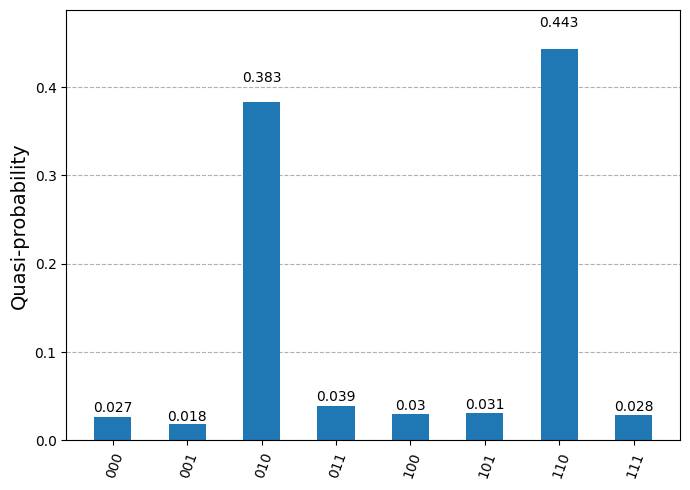
\includegraphics[width=0.6\textwidth]{hist1.png}
    \caption{Distribución de conteos enel hardware real.}
    \label{fig:grover_histogram}
\end{figure}

En al figura \ref{fig:grover_histogram} se puede ver como
la realidad se ajusta a la teoría. El sistema de qubits colapsó 
a 010 y 110, los cuales habían sido los estados
marcados. Esto con un porcentaje de desviación de 18.76\%.

Aunque el algoritmo de Grover es eficiente en teoría, su comportamiento en la 
práctica depende de la calidad del hardware cuántico. Los simuladores sirven 
para verificar que el circuito está bien construido, pero ejecutar en un backend 
real como el de IBm permite ver qué tan robusto es frente al ruido y qué tan 
factible sería usarlo 
en escenarios reales.


\subsection{Escenario 2: Estado Único}

En este caso se busca validar que el algoritmo de Grover identifica correctamente 
un único estado solución en un espacio pequeño. Es decir, llevarlo a su mínima 
expresión para estudiar su comportamiento base.

Se utilizan 3 qubits para representar el número 5 en decimal, que corresponde al 
estado \texttt{"101"} en binario. Según la teoría, el número óptimo de iteraciones 
es 2, ya que el valor de \( k \) se aproxima a 2.17.

\[
\theta = \arcsin\left( \sqrt{\frac{1}{8}} \right) = \arcsin\left( \frac{1}{\sqrt{8}} \right) \approx 0.361
\]

\[
k = \left\lfloor \frac{\pi}{4 \cdot \theta} \right\rfloor = \left\lfloor \frac{\pi}{4 \cdot 0.361} \right\rfloor = \left\lfloor \frac{\pi}{1.444} \right\rfloor \approx \left\lfloor 2.17 \right\rfloor = 2
\]


\begin{figure}[H]
    \centering
    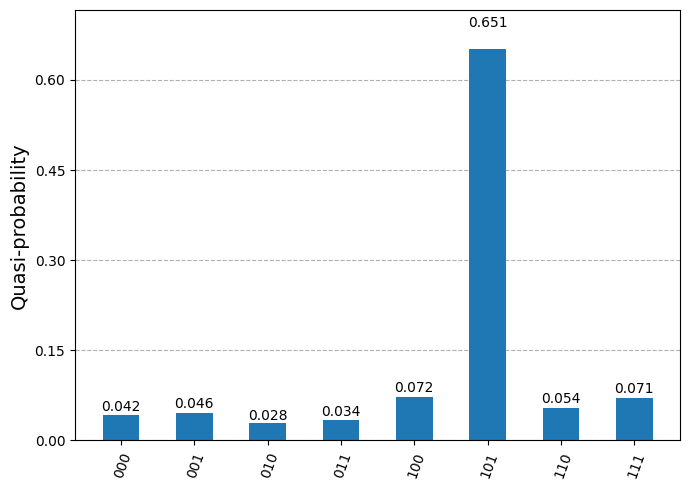
\includegraphics[width=0.6\textwidth]{hist2.png}
    \caption{Distribución de conteos en el hardware real.}
    \label{fig:grover_histogram2}
\end{figure}

En la figura \ref{fig:grover_histogram2} se puede ver cómo, al configurar el 
circuito para marcar un solo estado, el sistema cuántico real entrega una mayor 
cantidad de conteos en \texttt{101} al aplicar Grover. Esto valida que el algoritmo 
sigue funcionando incluso en presencia de ruido. De hecho, 
el porcentaje de desvicaicón estandar por el ruido es de 31.81\% lo cual es bueno.

Empíricamente se confirma la hipótesis: al tener solo una solución, se requieren 
más iteraciones para amplificar su probabilidad. Menos soluciones implican más 
rotación de amplitud. También es clave recordar que si se excede el número 
óptimo de iteraciones, la probabilidad de éxito empieza a disminuir nuevamente 
debido a interferencia cuántica.

Este escenario demuestra cómo la teoría se refleja de forma tangible en el 
comportamiento del hardware real, incluso con las limitaciones de ruido y 
decoherencia presentes.

 
\subsection{Escenario 3: Varios estados marcados con más qubits}

En este caso se busca validar si el algoritmo de Grover identifica correctamente 
dos estados solución dentro de un espacio de búsqueda más amplio, usando 4 qubits.

Los estados marcados corresponden a los números 6 y 11 en decimal, es decir,
\texttt{"0110"} y \texttt{"1011"} en binario.

El número óptimo de iteraciones se calcula según la fórmula teórica:

\[
k = \left\lfloor \frac{\pi}{4 \cdot \arcsin\left(\sqrt{\frac{2}{16}}\right)} 
\right\rfloor = 2
\]

Por tanto, se aplicaron dos iteraciones del operador de Grover en la ejecución 
sobre el hardware real de IBM.

\begin{figure}[H]
    \centering
    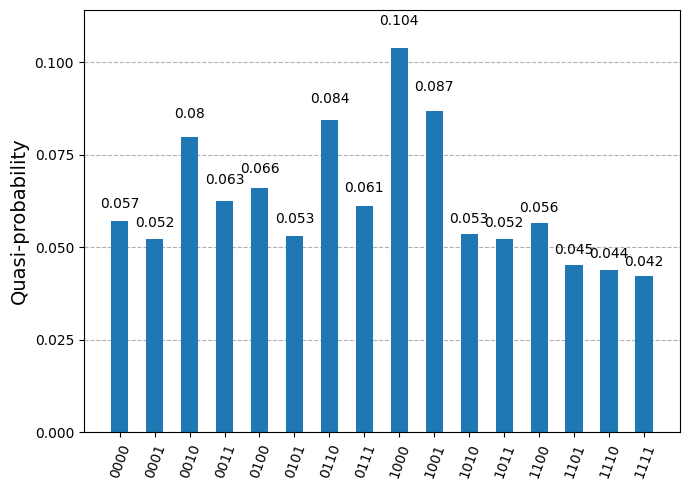
\includegraphics[width=0.6\textwidth]{hist3.png}
    \caption{Distribución de conteos en el hardware real con 2 iteraciones.}
    \label{fig:grover_histogram3}
\end{figure}

Sin embargo, en la figura \ref{fig:grover_histogram3} se observa que los estados 
marcados \texttt{0110} y \texttt{1011} no colapsan con mayor probabilidad, a 
diferencia de los resultados esperados y de lo visto en los escenarios 
anteriores (\ref{fig:grover_histogram} y \ref{fig:grover_histogram2}). 
En este caso, la probabilidad total desviada hacia estados no marcados fue del 86.33\%.

Ante esto, se propone la hipótesis de que, aunque teóricamente el número 
de iteraciones es correcto, la ejecución sobre hardware real específicamente 
una máquina cuántica compartida de IBM con 120 qubits introduce factores físicos como:

\begin{itemize}
    \item Ruido cuántico.
    \item Difusión imperfecta del operador de Grover.
    \item Limitaciones en la calibración o fidelidad de los qubits usados.
\end{itemize}

\begin{figure}[H]
    \centering
    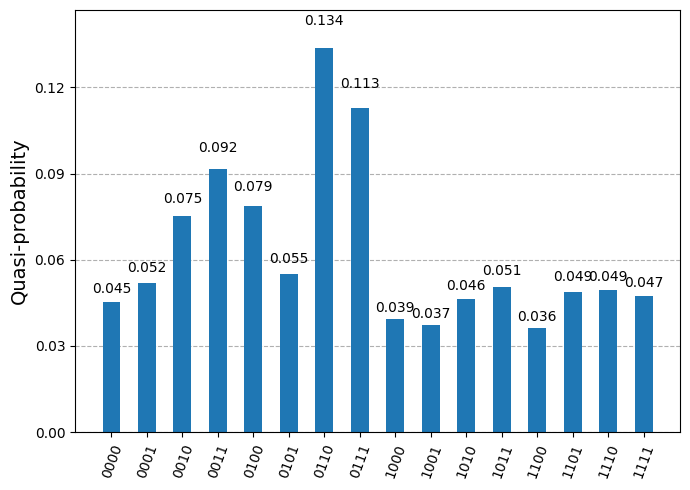
\includegraphics[width=0.6\textwidth]{hist3_a.png}
    \caption{Distribución de conteos con 1 iteración del operador de Grover.}
    \label{fig:grover_histogram3a}
\end{figure}

También se evaluó si el problema era el número de iteraciones. Al repetir el 
experimento con solo una iteración (figura \ref{fig:grover_histogram3a}), 
los estados marcados tampoco resultaron los más probables, y la desviación fue de 81.58\%. Esto permite descartar el exceso de iteraciones como causa principal del error.

Por lo tanto, se concluye que el bajo rendimiento en este escenario se 
debe principalmente al \textbf{ruido cuántico} y la \textbf{difusión imperfecta} 
en el backend físico utilizado.


\section{Referencias}
\renewcommand{\refname}{}

\begin{thebibliography}{9}

\bibitem{ref} \label{ref:Teo_Par}
A. Párraga, “Cómo se programa un ORDENADOR CUÁNTICO (bien explicado),” 
YouTube, 2021. [En línea]. Disponible en: 
\url{https://www.youtube.com/watch?v=eRlQdW1lgJE}.

\bibitem{ref} \label{ref:KetG} Ket.G, “Ket.G,” YouTube. 
[En línea]. Disponible en: \url{https://www.youtube.com/channel/UCedVPGH5fnWBmsR4oHVOX6w}.

\bibitem{ref} \label{ref:IBM_exp}
IBM Research, “Running an experiment in the IBM Quantum Experience,” 
YouTube, 2016. [En línea]. Disponible en: 
\url{https://www.youtube.com/watch?v=pYD6bvKLI_c}.

\bibitem{ref} \label{ref:IBM_QUAN} 
IBM Quantum, “IBM Quantum Platform,” \url{https://quantum.ibm.com/}.

\bibitem{ref} \label{ref:IBM_GROV} IBM Quantum. “Grover's algorithm.” 
IBM Quantum Learning, \url{https://learning.quantum.ibm.com/tutorial/grovers-algorithm}.


\end{thebibliography}

\end{document}